%%%%%%%%%%%%%%%%%%%%%%%%%%%%%%%%%%%%%%%%%
% Programming/Coding Assignment
% LaTeX Template
%
% This template has been downloaded from:
% http://www.latextemplates.com
%
% Original author:
% Ted Pavlic (http://www.tedpavlic.com)
%
% Note:
% The \lipsum[#] commands throughout this template generate dummy text
% to fill the template out. These commands should all be removed when 
% writing assignment content.
%
% This template uses a Perl script as an example snippet of code, most other
% languages are also usable. Configure them in the "CODE INCLUSION 
% CONFIGURATION" section.
%
%%%%%%%%%%%%%%%%%%%%%%%%%%%%%%%%%%%%%%%%%

%----------------------------------------------------------------------------------------
%	PACKAGES AND OTHER DOCUMENT CONFIGURATIONS
%----------------------------------------------------------------------------------------

\documentclass{article}

\usepackage{fancyhdr} % Required for custom headers
\usepackage{lastpage} % Required to determine the last page for the footer
\usepackage{extramarks} % Required for headers and footers
\usepackage[usenames,dvipsnames]{color} % Required for custom colors
\usepackage{graphicx} % Required to insert images
\usepackage{listings} % Required for insertion of code
\usepackage{courier} % Required for the courier font
\usepackage{lipsum} % Used for inserting dummy 'Lorem ipsum' text into the template

\usepackage{float}
\usepackage{amsfonts}
\usepackage{amsmath}
\usepackage{bm}

% Margins
\topmargin=-0.45in
\evensidemargin=0in
\oddsidemargin=0in
\textwidth=6.5in
\textheight=9.0in
\headsep=0.25in

\linespread{1.1} % Line spacing

% Set up the header and footer
\pagestyle{fancy}
\lhead{K. Holmbeck and D. Tonne} % Top left header
\chead{\hmwkClass\ : \hmwkTitle} % Top center head
\rhead{\firstxmark} % Top right header
\lfoot{\lastxmark} % Bottom left footer
\cfoot{} % Bottom center footer
\rfoot{Page\ \thepage\ of\ \pageref{LastPage}} % Bottom right footer
\renewcommand\headrulewidth{0.4pt} % Size of the header rule
\renewcommand\footrulewidth{0.4pt} % Size of the footer rule

\setlength\parindent{0pt} % Removes all indentation from paragraphs

%----------------------------------------------------------------------------------------
%	CODE INCLUSION CONFIGURATION
%----------------------------------------------------------------------------------------

\usepackage{color} %red, green, blue, yellow, cyan, magenta, black, white
\definecolor{mygreen}{RGB}{28,172,0} % color values Red, Green, Blue
\definecolor{mylilas}{RGB}{170,55,241}

\lstset{language=Matlab,%
    basicstyle=\ttfamily\footnotesize,breaklines=true
    %basicstyle=\footnotesize\color{red},
    breaklines=true,%
    xleftmargin=0.5in,
    %xrightmargin=0.25in,
    morekeywords={matlab2tikz},
    keywordstyle=\color{blue},%
    morekeywords=[2]{1}, keywordstyle=[2]{\color{black}},
    identifierstyle=\color{black},%
    stringstyle=\color{mylilas},
    commentstyle=\color{mygreen},%
    showstringspaces=false,%without this there will be a symbol in the places where there is a space
    numbers=left,%
    numberstyle={\tiny \color{black}},% size of the numbers
    numbersep=9pt, % this defines how far the numbers are from the text
    emph=[1]{for,end,break},emphstyle=[1]\color{blue}, %some words to emphasise
    %emph=[2]{word1,word2}, emphstyle=[2]{style},    
}


%----------------------------------------------------------------------------------------
%	DOCUMENT STRUCTURE COMMANDS
%	Skip this unless you know what you're doing
%----------------------------------------------------------------------------------------

% Header and footer for when a page split occurs within a problem environment
\newcommand{\enterProblemHeader}[1]{
%\nobreak\extramarks{#1}{#1 continued on next page\ldots}\nobreak
%\nobreak\extramarks{#1 (continued)}{#1 continued on next page\ldots}\nobreak
}

% Header and footer for when a page split occurs between problem environments
\newcommand{\exitProblemHeader}[1]{
\nobreak\extramarks{#1 (continued)}{#1 continued on next page\ldots}\nobreak
\nobreak\extramarks{#1}{}\nobreak
}

\setcounter{secnumdepth}{0} % Removes default section numbers
\newcounter{homeworkProblemCounter} % Creates a counter to keep track of the number of problems

\newcommand{\homeworkProblemName}{}
\newenvironment{homeworkProblem}[1][Problem \arabic{homeworkProblemCounter}]{ % Makes a new environment called homeworkProblem which takes 1 argument (custom name) but the default is "Problem #"
\stepcounter{homeworkProblemCounter} % Increase counter for number of problems
\renewcommand{\homeworkProblemName}{#1} % Assign \homeworkProblemName the name of the problem
\subsection{\homeworkProblemName} % Make a section in the document with the custom problem count
\enterProblemHeader{\homeworkProblemName} % Header and footer within the environment
}{
\exitProblemHeader{\homeworkProblemName} % Header and footer after the environment
}

\newcommand{\problemAnswer}[1]{ % Defines the problem answer command with the content as the only argument
\noindent\framebox[\columnwidth][c]{\begin{minipage}{0.98\columnwidth}#1\end{minipage}} % Makes the box around the problem answer and puts the content inside
}

\newcommand{\homeworkSectionName}{}
\newenvironment{homeworkSection}[1]{ % New environment for sections within homework problems, takes 1 argument - the name of the section
\renewcommand{\homeworkSectionName}{#1} % Assign \homeworkSectionName to the name of the section from the environment argument
\subsection{\homeworkSectionName} % Make a subsection with the custom name of the subsection
\enterProblemHeader{\homeworkProblemName\ [\homeworkSectionName]} % Header and footer within the environment
}{
\enterProblemHeader{\homeworkProblemName} % Header and footer after the environment
}


%----------------------------------------------------------------------------------------
%   NAME AND CLASS SECTION
%----------------------------------------------------------------------------------------

\newcommand{\hmwkTitle}{Homework\ 2} % Assignment title
\newcommand{\hmwkDueDate}{Tuesday,\ March\ 6,\ 2018} % Due date
\newcommand{\hmwkClass}{Math\ 521} % Course/clas
\newcommand{\hmwkAuthorName}{Kristin Holmbeck} % Your name

%----------------------------------------------------------------------------------------
%   TITLE PAGE
%----------------------------------------------------------------------------------------

\title{
\textmd{\textbf{\hmwkClass \ \hmwkTitle}}\\
\normalsize\vspace{0.1in}\small{Due\ on\ \hmwkDueDate}\\
\vspace{0.1in}
\vspace{0.2in}
}

\author{\textbf{\hmwkAuthorName}}
\date{} % Insert date here if you want it to appear below your name

%----------------------------------------------------------------------------------------

\begin{document}

\maketitle

%----------------------------------------------------------------------------------------
%   TABLE OF CONTENTS
%----------------------------------------------------------------------------------------

%\setcounter{tocdepth}{1} % Uncomment this line if you don't want subsections listed in the ToC
\vspace{0.75in}
\tableofcontents
\listoffigures
\newpage

%----------------------------------------------------------------------------------------
%   PROBLEM 1
%----------------------------------------------------------------------------------------

% To have just one problem per page, simply put a \clearpage after each problem

\begin{section}{Theory}

\begin{homeworkSection}{1. Unique Decomposition}

Let $W_1, W_2$ be vector subspaces and $W=W_1+W_2, W_1 \neq W_2$. Show, by giving an example, that the decomposition of a vector $\bm{x} \in W$ is not unique.

\problemAnswer{
    The requirements for a subspace $\hat{W}$ include :
    \begin{itemize}
        \item The zero vector is in $\hat{W}$
        \item If $\bm{u}, \bm{v} \in \hat{W}$, then $\bm{u}+\bm{v} \in \hat{W}$
        \item If $\bm{u} \in \hat{W}, c \in \mathbb{R}, c\bm{u} \in \hat{W}$
    \end{itemize}
    If we let $W = \{\begin{bmatrix} x && y && 0 \end{bmatrix}^T \ni x,y \in \mathbb{R} \} \subset \mathbb{R}^3$, then we can decompose $W$ into $W_1 = \{\begin{bmatrix} x && 0 && 0 \end{bmatrix}^T \ni x,y \in \mathbb{R} \}$ and $W_2 = \{\begin{bmatrix} x && y && 0 \end{bmatrix}^T \ni x,y \in \mathbb{R} \}$. Then, we can express a vector $\bm{x} \in W$ non-uniquely. For example:
    \begin{align*}
        \bm{x} = \begin{bmatrix} 2 \\ 10 \\ 0 \end{bmatrix} 
            = \begin{bmatrix} 1 \\ 0 \\ 0 \end{bmatrix} + \begin{bmatrix} 1 \\ 10 \\ 0 \end{bmatrix} 
            = \begin{bmatrix} 2 \\ 0 \\ 0 \end{bmatrix} + \begin{bmatrix} 0 \\ 10 \\ 0 \end{bmatrix}
    \end{align*}
}

\end{homeworkSection}

\begin{homeworkSection}{2. Matrix Bases}
Consider the matrix
\begin{align*}
    A = \begin{bmatrix} 1 && -1 \\ 2 && -2 \\ 3 && -3 \end{bmatrix}
\end{align*}
Determine bases for the column space, row space, null space, and left null space of $A$.
\\
\\

\problemAnswer{ 

\begin{itemize}

\item The column space of $A$ is the linearly independent columns in $A$. Since the second column is a scalar multiple of the first (by -1), the column space of $A$ is: \\ span$ \left \{ \begin{bmatrix} 1 \\2 \\ 3 \end{bmatrix} \right \} $.

\item The row space of $A$ is the linearly independent rows of $A$. Notice that rows 2 and 3 are scalar multiples of the first row. Hence, the row space is: \\ span$ \left \{ \begin{bmatrix} 1 \\ -1 \end{bmatrix} \right \} $.
\end{itemize}
}

\problemAnswer{ 

\begin{itemize}
\item The null space of $A$ includes the vectors that solve $Ax = \bm{0}$. Then it is easy to see that $A \begin{bmatrix} x_1 \\ x_1 \end{bmatrix} = \bm{0}$ solves this. In other words, \\ null space of $A$ = span $\left\{ \begin{bmatrix} 1 \\ 1 \end{bmatrix} \right \}$.

\item The \textit{left} null space of $A$ are the vectors that solve $x^TA = 0$. \\
$\begin{bmatrix} x_1 & x_2 && x_3 \end{bmatrix} \begin{bmatrix} 1 && -1 \\ 2 && -2 \\ 3 && -3 \end{bmatrix} = \begin{bmatrix} x_1+2x_2+3x_3 && -x_1-2x_2-3x_3 \end{bmatrix} = \bm{0}$ \\
The most direct way to solve this is to convert $ [ A \quad | \quad I_{3}  ] $ to reduced-row echelon form. Performing this calculation, we obtain the basis for the left null space: \\
span = $\left \{ \begin{bmatrix} 1 \\ 0 \\ -\frac{1}{3}\end{bmatrix},
                \begin{bmatrix} 0 \\ 1 \\ -\frac{2}{3}\end{bmatrix} \right \}
        $
\end{itemize}
}

\end{homeworkSection}


\begin{homeworkSection}{3. Projections}
Let $V = \mathbb{R}^3$, let 
\begin{align*}
    u^{(1)} = \begin{bmatrix} 1 \\ 2 \\ 0 \end{bmatrix}, 
    u^{(2)} = \begin{bmatrix} -1 \\ 0 \\ 1 \end{bmatrix}, 
    x = \begin{bmatrix} 0 \\ 2 \\ 1 \end{bmatrix},
\end{align*}
and define $W = \text{span}(u^{(1)}, u^{(2)})$. Find the orthogonal projection of $x$ onto $W$. Also find the projection matrix $\mathbb{P}$ associated with this mapping.
\\
\\
\problemAnswer{
    For orthogonal projections, the Gram-Schmidt process is used -- a method for generating an orthonormal basis from a set of vectors. Using the Gram-Schmidt algorithm (in the Code section of this document), we obtain the basis vectors:
    \begin{align*}
        e^{(1)} = \frac{1}{\sqrt{5}} \begin{bmatrix} 1 \\ 2 \\ 0 \end{bmatrix}, \qquad
        e^{(2)} = \frac{1}{3\sqrt{5}} \begin{bmatrix} -4 \\ 2 \\ 5 \end{bmatrix}
    \end{align*}
    A projection matrix $\mathbb{P}_i$ onto $e^{(i)}$, is given by $e^{(i)} {e^{(i)}}^T$. From this, we have the two projection matrices for the basis vectors above:
    \begin{align*}
        \mathbb{P}_1 &= \frac{1}{5} \begin{bmatrix} 1 && 2 && 0 \\ 2&& 4 && 0 \\ 0 && 0 && 0 \end{bmatrix} \\ 
        \mathbb{P}_2 &= \frac{1}{45} \begin{bmatrix} 16 && -8 && -20 \\ -8 && 4 && 10 \\ -20 && 10 && 25 \end{bmatrix} \\ 
        \text{then the total projection is: }
        \mathbb{P} &= \mathbb{P}_1 + \mathbb{P}_2 = \frac{1}{9} \begin{bmatrix} 5 && 2 && -4 \\ 2 && 8 && 2 \\ -4 && 2 && 5 \end{bmatrix}
    \end{align*}
    \\
    Lastly, note that $x = u^{(1)} + u^{(2)}$, in other words $x \in W$, so we expect the orthogonal projection of $x$ onto $W$ to be itself. Indeed it is, as $\mathbb{P}x = x$.
}

\end{homeworkSection}

\begin{homeworkSection}{4. Orthonormal Basis Vectors}
Reconsider Problem 3. Find vectors such that $x = UU^Tx$ and $x \neq UU^Tx$ where the matrix $U$ consists of the orthonormal basis vectors of $W$ from Problem 3.
\\
\\
\problemAnswer{
    Note that $UU^T = \mathbb{P}$ since
    \begin{align*}
        U &= \left[ e^{(1)} \quad e^{(2)} \right ] \\
        UU^T &= \begin{bmatrix} e^{(1)} && e^{(2)} \end{bmatrix}
                \begin{bmatrix} {e^{(1)}}^T \\  {e^{(2)}}^T \end{bmatrix}  \\
        &= \left[ e^{(1)}{e^{(1)}}^T + e^{(2)}{e^{(2)}}^T \right ] 
        = \mathbb{P} \qquad \text{by construction}
    \end{align*}
    As stated previously, the given vector $x = \left[ 0, 2, 1 \right]^T$ solves $\mathbb{P}x=x$. In order to find a $y \ni \mathbb{P}y \neq y$, we will use a $y \notin W$. Let $y = \left [ 1,1,1 \right ]^T$. Then $\mathbb{P}y = \frac{1}{3} \left [ 1,4,1 \right ]^T \neq y$.
}
\end{homeworkSection}

\begin{homeworkSection}{5. SVD}
Determine the SVD of the data matrix
\begin{align*}
    A = \begin{bmatrix} -2 && -1 && 1 \\ 0 && -1 && 0 \\ -1 && 1 && 2 \\ 1 && -1 && 1 \end{bmatrix}
\end{align*}
and compute rank-one, -two, and -three approximations to $A$.
\\
\\
\problemAnswer{
    We will compute the SVD of $A$ "manually", that is, we will show the steps for how to compute the SVD, but leave the heavy lifting to \textsc{Matlab}. First, consider the characteristic equation for $A^TA$:
    \begin{align*}
        A^TA &= \begin{bmatrix} 6 && 0 && -3 \\
                               0 && 4 && 0 \\
                               -3 && 0 && 6 \end{bmatrix} \\
        \rho(A^TA)  &= | A^TA - \lambda I | = - \lambda^3 + 16\lambda^2 - 75\lambda + 108 = 0 \\
             0  &= (\lambda-9)(\lambda - 4)(\lambda-3) \qquad \text{by long division} \\
        \lambda &= \left \{ 9, 4, 3  \right \}
    \end{align*}
    Since our $A$ matrix is 4x3, $\Sigma$ will be the same size.
    \begin{align*}
        \Sigma = \begin{bmatrix} \sqrt{9} && 0 && 0 \\ 
                                0 && \sqrt{4} && 0 \\
                                0 && 0 && \sqrt{3} \\
                                0 && 0 && 0
                \end{bmatrix}
        &= \begin{bmatrix} 3 && 0 && 0 \\ 
                                0 && 2 && 0 \\
                                0 && 0 && 1.7321 \\
                                0 && 0 && 0
                \end{bmatrix}
    \end{align*}
}
\problemAnswer{
    We obtain the null spaces corresponding to the matrix $(A^TA-\lambda I)$, and use these to form the $V$ matrix. 
    \begin{align*}
        V = \begin{bmatrix} -0.7071 && 0 && -0.7071 \\
                            0       && -1 && 0 \\
                            0.7071  && 0 && -0.7071
            \end{bmatrix}
    \end{align*}

    Lastly, we begin construction of the $U$ matrix using $u_i = \frac{1}{\sigma_i} Av_i$ as the first several column vectors. 

    \begin{align*}
        AV\Sigma^{-1} = \hat{U} = \begin{bmatrix} 
                0.4082 &&   0.5000  &&  0.7071  && 0 \\
                     0 &&   0.5000  &&       0  && 0 \\
               -0.4082 &&  -0.5000  &&  0.7071  && 0 \\
               -0.8165 &&   0.5000  &&       0  && 0 \\
            \end{bmatrix}
    \end{align*}

    The last column of $U$ can be obtained via the same eigenvalue method on $AA^T$. We know that this corresponds to an eigenvalue of zero, so by computing the null space of $AA^T$, we obtain the full matrix for $U$:
    \begin{align*}
        U = \begin{bmatrix} 
                0.4082 &&   0.5000  &&  0.7071  && -0.2887 \\
                     0 &&   0.5000  &&       0  &&  0.8660 \\
               -0.4082 &&  -0.5000  &&  0.7071  &&  0.2887 \\
               -0.8165 &&   0.5000  &&       0  &&  -0.2887 \\
            \end{bmatrix}
    \end{align*}
    Then $A$ can be decomposed into $A = U \Sigma V^T$ by the singular value decomposition theorem. Checking this with \textsc{Matlab} yields the same decomposition. (Note: the decomposition is not \textit{exactly} the same, but differs in placement of some negative signs.)
    \\
    \\
    In order to determine low-rank approximations, we will denote the rank-$k$ approximation to $A$, called $A_k$, by:
    \begin{align*}
        A_k = \begin{bmatrix} u_{11} && \cdots && u_{1k} \\ \vdots && \ddots && \vdots \\ u_{k1} && \cdots && u_{kk} \end{bmatrix}
        \begin{bmatrix} s_{11} &&  && 0 \\  && \ddots &&  \\ 0 &&  && s_{kk} \end{bmatrix}
        \begin{bmatrix} v_{11} && \cdots && v_{1k} \\ \vdots && \ddots && \vdots \\ v_{k1} && \cdots && v_{kk} \end{bmatrix}^T
    \end{align*}
    \begin{align*}
        A_1 = \begin{bmatrix} -1.5 && 0 && 1.5\\ 
        0 && 0 && 0\\ 
        -1.5 && 0 && 1.5\\ 
        0 && 0 && 0\end{bmatrix} \quad 
        A_2 = \begin{bmatrix} -1.5 && -1 && 1.5\\ 
        0 && -1 && \epsilon \\ 
        -1.5 && 1 && 1.5\\ 
        0 && -1 && \epsilon \end{bmatrix}  \quad
        A_3 = \begin{bmatrix} -2 && -1 && 1\\ 
        0 && -1 && \epsilon \\ 
        -1 && 1 && 2\\ 
        1 && -1 && 1\end{bmatrix}
    \end{align*}
    Where $\epsilon = \mathcal{O}(1e-15)$, machine-precision zero with roundoff error.
    An interesting result from this is the spectral norm of the residual $A-A_k$ is equal to the $(k+1)$-th singular value of $A$. This theorem comes from \cite{stanford}.
    \begin{align*}
        || A - A_1 ||_2 &= 2 = S_{22}\\
        || A - A_2 ||_2 &= 1.7321 = S_{33}\\
        || A - A_3 ||_2 &= 0  \qquad \qquad \text{is exact (up to machine precision), as expected}\\
    \end{align*}
}
\end{homeworkSection}

\end{section}

%----------------------------------------------------------------------------------------
%   PROBLEM 2
%----------------------------------------------------------------------------------------
\begin{section}{Computing}

\begin{homeworkSection}{1. Kohonen's Novelty Filter }
Consider the training set consisting of the following three patterns consisting of 5 $\times$ 4 arrays of black squares (Figure \ref{fig:training}). Using Kohonen's novelty filter, find and display (in terms of an image) the novelty in the pattern from Figure \ref{fig:pattern}.

\begin{figure}[H]
\centering

\includegraphics[width=0.75\columnwidth]{../data/kohonen_training}
\caption{Training Data for Kohonen}
\label{fig:training}
\end{figure}


\begin{figure}[H]
\centering

\includegraphics[width=0.35\columnwidth]{../data/pattern}
\caption{Pattern to compare with training set from Figure \ref{fig:training}}
\label{fig:pattern}
\end{figure}

Proceed by assuming that the black square entries have numerical value one and the blank entries have numerical value zero. Concatenate the columns of each pattern to make vectors in $\mathbb{R}^{20}$. Does your result make sense? Why or why not?

\problemAnswer{
    We can decompose a vector $x$ into its orthogonal projection and the complement of its orthogonal projection, i.e. $x = w + w^T = \mathbb{P}x + (I-\mathbb{P})x$. From Kohonen \cite{kohonen}, the novelty is the orthogonal complement, $w^T$.
    \\
    \\
    In order to calculate the novelty, we find an orthonormal basis for the first three patterns. We create a matrix of size (20 x 3), and obtain an orthonormal basis $W$. The projection matrix then becomes $\mathbb{P} = WW^T$, and the novelty is then $(I-\mathbb{P})x$, where $x$ is the (20 x 1) vector obtain from concatenating the columns of the pattern in Figure \ref{fig:pattern}. 
    \\
    \\
    This gives us the novelty shown in Figure \ref{fig:novelty}, corresponding to the matrix below:
    \\
    \begin{minipage}{.5\textwidth}
        \begin{align*}(I-\mathbb{P})x = w^T =  \begin{bmatrix}
                0  &&  0  &&  0  &&  0 \\
                     0  &&       1  &&       0  && 0 \\
                     0  &&       1  &&       0  && 0 \\
                     0  &&       1  &&       0  && 0 \\
                0 && 0 && 0 && 0
        \end{bmatrix}\end{align*}
    \end{minipage}
    \begin{minipage}{.5\textwidth}
        \begin{figure}[H]
        \centering
        
\includegraphics[width=0.35\columnwidth]{../data/novelty}
        \caption{Novelty from Kohonen's filter}
        \label{fig:novelty}
        \end{figure}
    \end{minipage}
    \\
    \\
    \\
    Does this result make sense? Our comparison data is a linear combination of the training data, other than the vertical column appearing in the middle of the matrix. It makes sense then that our novelty, or difference, appears in that column.
}

\end{homeworkSection}


\begin{homeworkSection}{2. SVD on a boolean matrix}
Compute the SVD of the matrix $A$ whose entries come from the first pattern in Figure \ref{fig:training} and display (in terms of an image) the reconstructions $A_1, A_2, A_3, A_4$. Again, treat the squares as ones and the blanks as zeros. Your reconstructions should be matrices with numerical values. Interpret your results.

\problemAnswer{
    \begin{align*}
        A &= \begin{bmatrix}
             1   &&  1  &&   1  &&   1 \\
             0   &&  1  &&   0  &&   1 \\
             0   &&  1  &&   0  &&   1 \\
             0   &&  1  &&   0  &&   1 \\
             1   &&  1  &&   1  &&   1 \\
        \end{bmatrix}
        = U S V^T  \qquad \text{computed via \textsc{Matlab}}
    \end{align*}
    In particular, note the construction of the singular value matrix
    \begin{align*}
        S &= \begin{bmatrix}
            3.4641 && 0 && 0 && 0 \\
            0 && 1.4142 && 0 && 0  \\
            0 &&  0 && 0 && 0 \\0 &&  0 && 0 && 0 \\
        \end{bmatrix} 
    \end{align*}
    With this knowledge, we expect the rank-2 and greater approximations to be "very close" ($||A-A_k||$ is small) to the original matrix $A$. Indeed, this is the case
    \begin{align*}
        A_1 &= \begin{bmatrix} 0.6 && 1.2 && 0.6 && 1.2\\ 
        0.4 && 0.8 && 0.4 && 0.8\\ 
        0.4 && 0.8 && 0.4 && 0.8\\ 
        0.4 && 0.8 && 0.4 && 0.8\\ 
        0.6 && 1.2 && 0.6 && 1.2\end{bmatrix} \\ 
        A_2 = A_3 = A_4 &= \begin{bmatrix} 1 && 1 && 1 && 1\\ 
        \epsilon && 1 && \epsilon && 1\\ 
        \epsilon && 1 && \epsilon && 1\\ 
        \epsilon && 1 && \epsilon && 1\\ 
        1 && 1 && 1 && 1\end{bmatrix} \\ 
        ||A- A_1|| &= \sqrt(2) = 1.4142 \\
        ||A- A_2|| &=  ||A- A_3|| = ||A- A_4|| = \epsilon \\
    \end{align*}
    For brevity, let's look at the image representation of just $A_1$, which we know is not "good" compared to the other, higher-rank approximations.
    \begin{figure}[H]
    \centering
    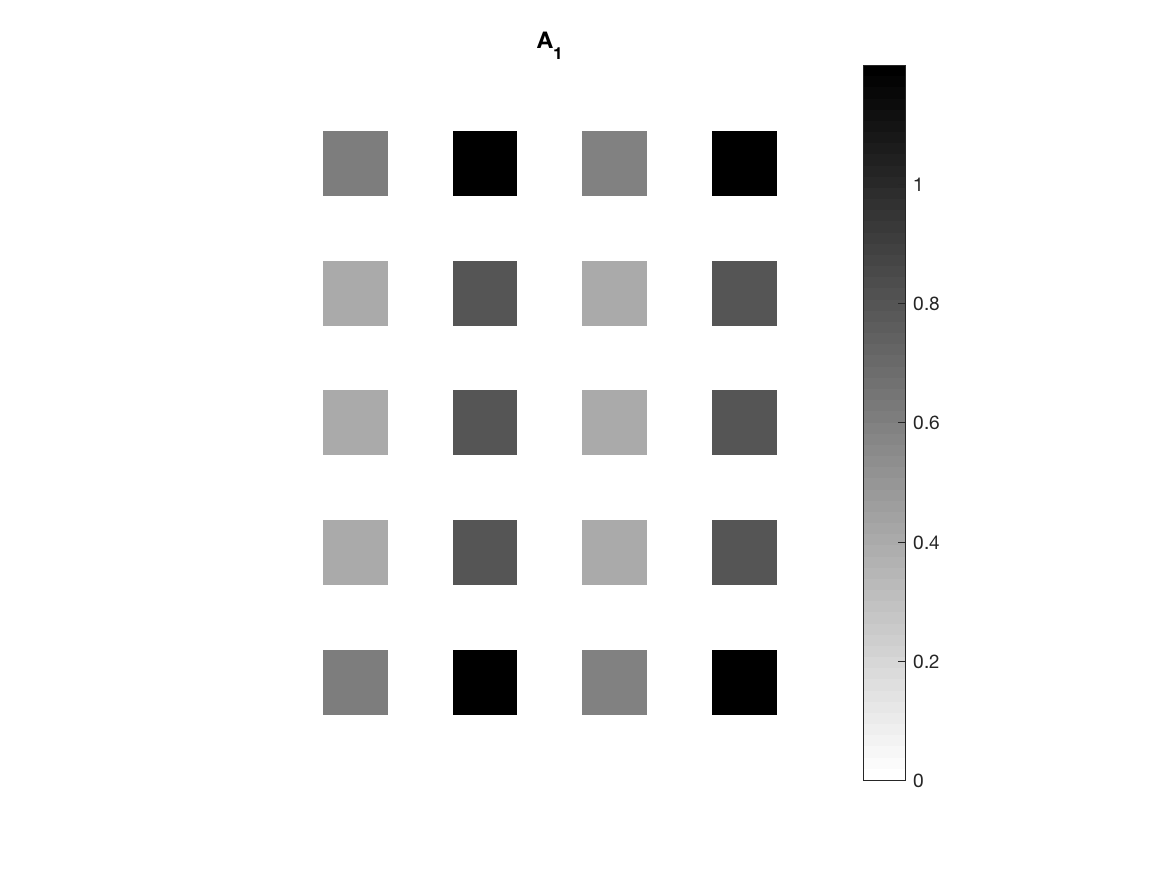
\includegraphics[width=0.35\columnwidth]{../data/Prob2_1}
    \caption{Reconstruction of $A$ by $A_1$}
    \label{fig:p2_1}
    \end{figure}
    You can see some residuals in spaces where we expect/want the matrix to be zero. Since this is a rank-1 approximation and $\sigma_1$ is not much greater than $\sigma_2$, the rank-1 approximation is not expected to be accurate.
}
\end{homeworkSection}


\begin{homeworkSection}{3. (a) SVD on a higher-resolution image}


\begin{figure}[H]
\centering
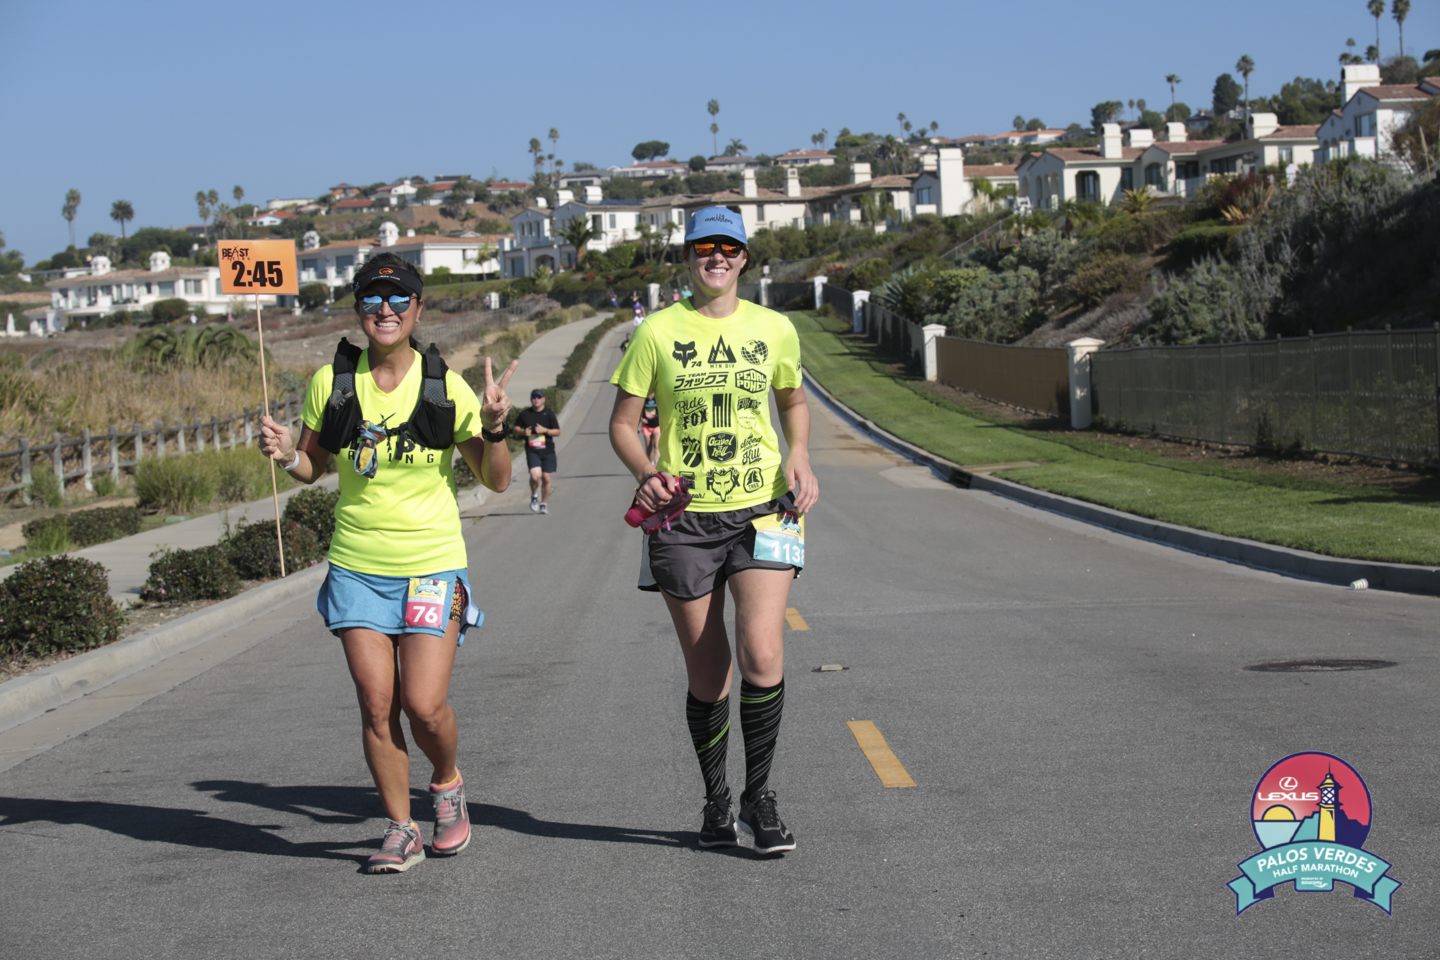
\includegraphics[width=0.95\columnwidth]{../data/testim}
\caption{Test Image: Palos Verdes Half Marathon (960 $\times$ 1440)}
\label{fig:myim}
\end{figure}


Computing the cumulative energy $E$ via $E_k = \cfrac{\Sigma_{i=1}^{k} \sigma_i^2}{\Sigma_{i=1}^{k} \sigma_i^2}$ with $r=$ rank(image) and $k \leq r$, we obtain the \textit{numerical rank} of the image in Figure \ref{fig:myim} as 6; the number of singular values required to retain at least 95\% of the energy in the original image. The cumulative energy is shown in Figure \ref{fig:energy}. What this actually looks like in terms of reconstruction is shown in Figure \ref{fig:rank_6}.

\begin{figure}[H]
\centering
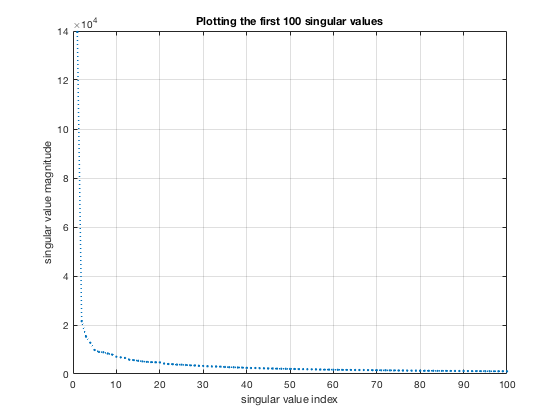
\includegraphics[width=0.75\columnwidth]{../data/SVD_dist}
\caption{Singular Value Distribution (first 100 of 960) of Figure \ref{fig:myim}}
\label{fig:svd_dist}
\end{figure}

\begin{figure}[H]
\centering
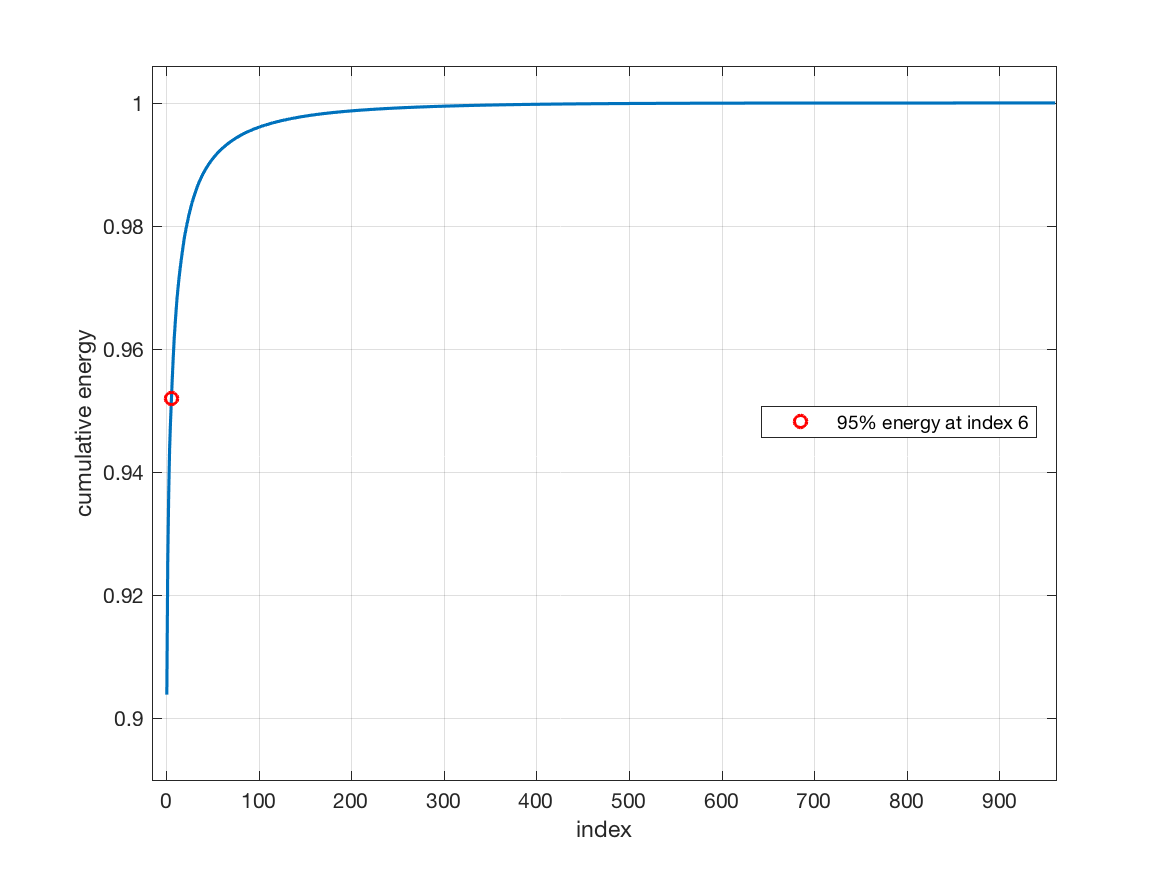
\includegraphics[width=0.75\columnwidth]{../data/cumulative_energy}
\caption{Cumulative Energy of Figure \ref{fig:myim}}
\label{fig:energy}
\end{figure}

\begin{figure}[H]
\centering
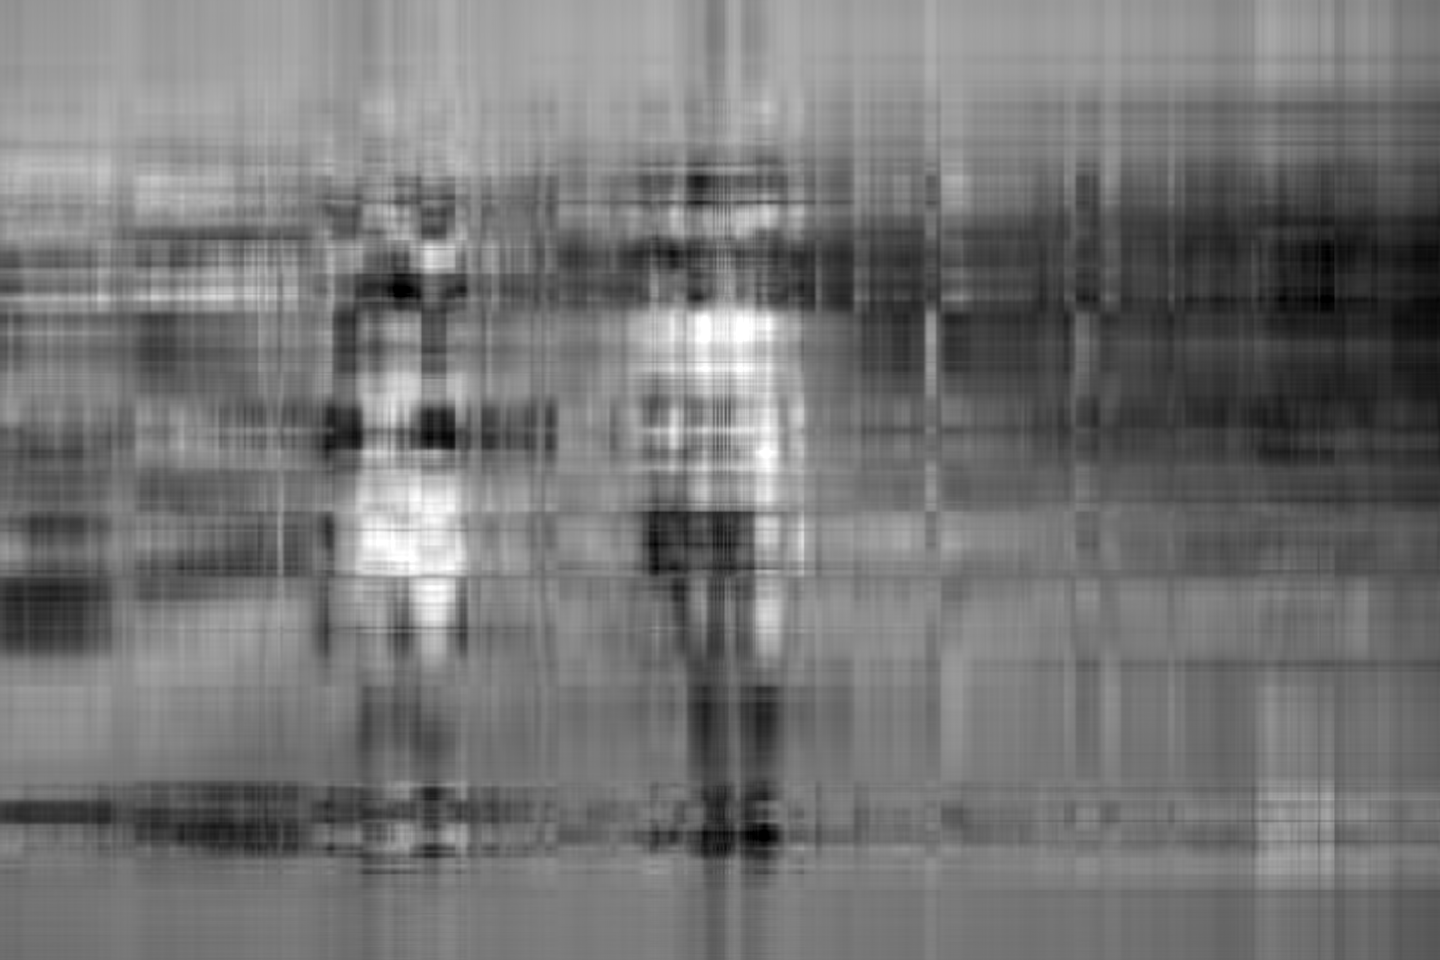
\includegraphics[width=0.90\columnwidth]{../data/rank_6_approx}
\caption{Rank-6 Approximation of Figure \ref{fig:myim}}
\label{fig:rank_6}
\end{figure}

In fact, in order to retain 99\% of the energy, we need a rank-47 approximation. The resulting reconstruction is given in Figure \ref{fig:rank_47}.

\begin{figure}[H]
\centering
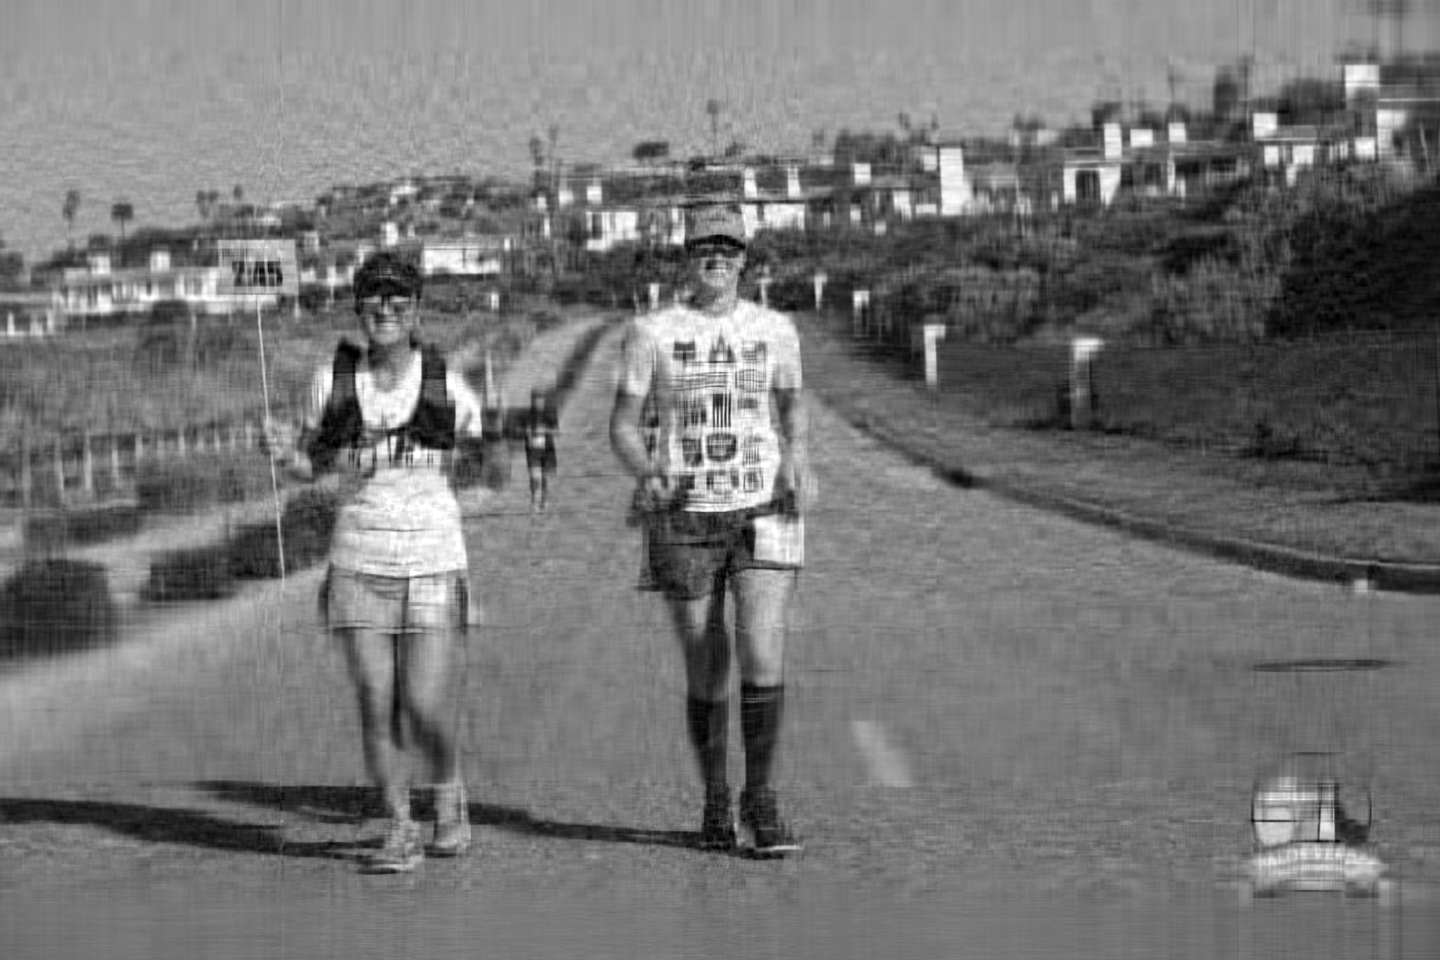
\includegraphics[width=0.90\columnwidth]{../data/rank_47_approx}
\caption{Rank-47 Approximation of Figure \ref{fig:myim}}
\label{fig:rank_47}
\end{figure}

\end{homeworkSection}

\begin{homeworkSection}{3. (b) Lower-Rank Approximations}

Recall that the relative error of a rank-$k$ approximation is given by $\sigma_{k+1} / \sigma_k$. As show in Figure \ref{fig:rank_approxs}, the relative errors $\tau_i$ are:
\begin{align*}
    \tau_{10} &= 0.9579 \\ 
    \tau_{50} &= 0.9798 \\ 
    \tau_{100} &= 0.9816 \\ 
    \tau_{200} &= 0.9954 \\ 
\end{align*}

\begin{figure}[H]
\centering
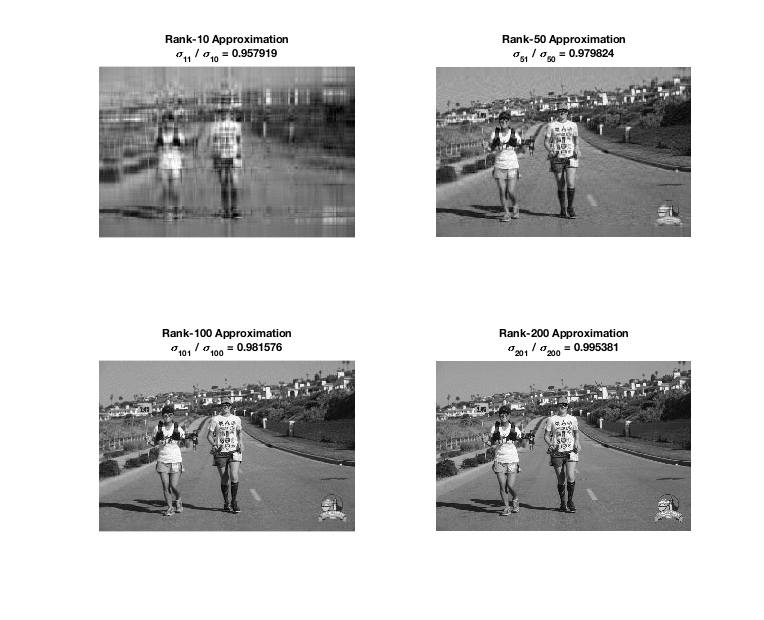
\includegraphics[width=0.9999\columnwidth]{../data/lower_rank_approxs}
\caption{Lower-Rank Approximations of Figure \ref{fig:myim}}
\label{fig:rank_approxs}
\end{figure}


\end{homeworkSection}

\end{section}


%----------------------------------------------------------------------------------------
\newpage

\appendix

\section{Code}\label{code}

\subsection{Gram-Schmidt} \label{code:gram_schmidt}

\lstinputlisting{../Kristin_Holmbeck_HW2_GramSchmidt.m}


\begin{thebibliography}{10}
    \bibitem{chang}
    Chang, Jen-Mei. \textit{Matrix Methods for Geometric Data Analysis and Recognition}. 2014.

    \bibitem{kohonen}
    T. Kohonen. Self-Organization and Associative Memory. Springer-Verlag, Berlin, 1984.

    \bibitem{stanford}
    Manning, Christopher D. and Raghavan, Prabhakar, and Schütze, Hinrich.
    \textit{Introduction to Information Retrieval}. Cambridge University Press. 2008. 
    [online] Available at: https://nlp.stanford.edu/IR-book/html/htmledition/low-rank-approximations-1.html [Accessed 25 Feb. 2018].

\end{thebibliography}

\end{document}
